\subsection{Persiapan \textit{kubernetes cluster}}
\label{subsec:persiapan-kubernetes-cluster}

Tahapan ini merupakan tahapan persiaspan sebelum proses \textit{development}. Pada tahapan ini dibuat kubernetes \textit{cluster} pada komputer lokal dengan kakas \textit{kind}. \textit{Cluster} yang dibuat memiliki 4 nodes dengan spesifikasi 1 \textit{master node} dan 3 \textit{worker node}. Digunakan \textit{command} kind create cluster --config cluster.yaml dengan file konfigurasi yang dapat dilihat pada gambar \ref{fig:konfigurasi-pembuatan-cluster}. Setelah berhasil di \textit{apply}, muncul 4 buah kontainer yang dapat berfungsi sebagai \textit{kubernetes cluster} seperti pada gamabar \ref{fig:hasil-cluster-kind}.

\begin{figure}[htbp]
    \centering
    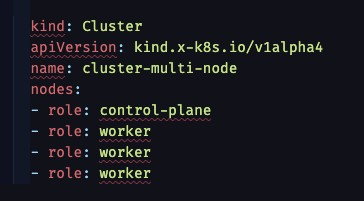
\includegraphics[width=1\textwidth]{resources/appendix/pembuatan-cluster.jpg}
    \caption{Konfigurasi Pembuatan \textit{Kubernetes Cluster} dengan \textit{Kind}}
    \label{fig:konfigurasi-pembuatan-cluster}
\end{figure}

\begin{figure}[htbp]
    \centering
    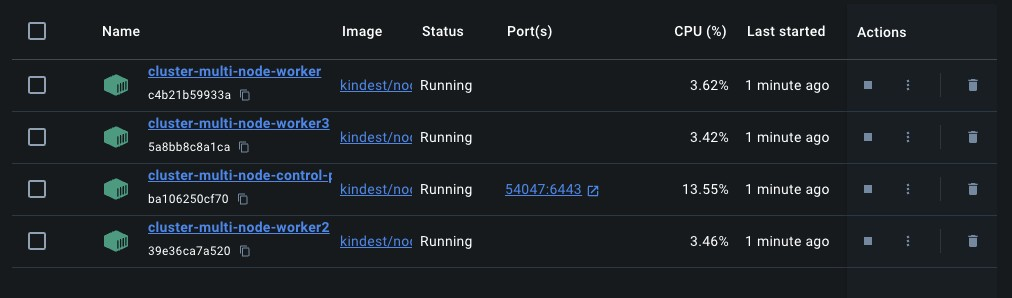
\includegraphics[width=1\textwidth]{resources/chapter-4/cluster-kind.jpg}
    \caption{Hasil \textit{Kubernetes Cluster} Dengan Kakas \textit{Kind}}
    \label{fig:hasil-cluster-kind}
\end{figure}

\pagebreak